\documentclass[conference,9pt]{IEEEtran}
\usepackage{xcolor}
\usepackage{cite}
\usepackage{epsfig}
\usepackage{amssymb}
\usepackage{amsmath}
\usepackage{graphicx}
\graphicspath{ {./} }

\begin{document}
\title{Practical 2b}

\author{
\IEEEauthorblockN{Albert Acebron}
\IEEEauthorblockA{NIU: 1458626}
}


% make the title area
\maketitle
\begin{abstract}
This practical will continue on applying ML to estimate the phase of a signal
\end{abstract}



%----------------------------------------------------------------
% SECTION #1 
\section{Introduction}

\section{Questions}

\subsection{Question 1}
In this question we'll have to force the variance of the noise to be 1.

Now, the definition of variance is $var=E[(X-\mu)^2]$, where $\mu$ is the mean of $X$, and because $X$ is gaussian noise, it's mean will be 0, so $var=E[X^2]$.

Forcing $var=1$ we get to the point where we need to force the expected value of $X^2$ to be one, and one way to do it is by forcing all $X$ to just be $1$. Given that this is the easiest solution and it can be applied with a single scaling factor we'll just put it in place:

Given $x$, a realization of $X$, if we divide it by itself we'll ensure that the resulting value is $1$, so we'll apply that procedure to all the values of $X$. In other words, we will divide these values by their absolute value in order to force their variance to be one.

If we'd rather use a single constant that would also be possible, but given that the solution provided is slightly easier to implement we opted for this one.

\subsection{Question 2}
We are only interested in finding the maximum (minimum in the case of equation 1.2) and because log is a strictly increasing function the minimum/maximum of these two functions will be in the same position, thus we only need to find one of these. In other words if we find an $x$ such that $-ln(f(x))$ is a minimum then $f(x)$ will be a maximum and thus we will have achieved our objective.

The reason why we are doing this transformation is because when we differentiate our function to obtain the minimum/maximum we get an expression that's much easier to work with if we apply the negative log transformation before (if we didn't we'd have to carry an exponetial and we wouldn't be able to cancel constant terms).

\subsection{Question 3}
The concrete value of $\theta$ is directly defined by equation 1.4 and we can get it by simply substituting several variables into it and evaluating the result, as we will do in the following exercises.

\subsection{Question 4}
Let's start by generating the samples with $\theta=1$:

\begin{verbatim}
  fd=0.25;
  A=5;
  N=10000;
  n=(1:N)';
  noise=randn(N, 1) + randn(N, 1)*i;
  noise=noise./abs(noise);
  x=A*cos(2*pi*fd.*n + 1) + noise;
\end{verbatim}

Define an estimator routine:

\begin{verbatim}
function [theta] = estimate(n, x, fd)
  upper=sum(x.*sin(2*pi*fd*n));
  lower=sum(x.*cos(2*pi*fd*n));
  theta=-atan(upper./lower);
end
\end{verbatim}

And apply it:

\begin{verbatim}
  theta1 = estimate(n(1:100), x(1:100), fd)
    1.0170 - 0.0457i
  theta2 = estimate(n(1:1000), x(1:1000), fd)
    1.0027 - 0.0096i
  theta3 = estimate(n(1:10000), x(1:10000), fd)
    1.0016 + 0.0001i
\end{verbatim}

We can appreciate that generally all predictions are pretty accurate but as $N$ grows the accuracy improves.

\subsection{Question 5}
We will create the plot with the following code:
\begin{verbatim}
  N=1000;
  n=(1:N)';
  thetas = zeros(1000, 1);
  for c=1:1000
    noise=randn(N, 1) + randn(N, 1)*i;
    noise=noise./abs(noise);
    x=A*cos(2*pi*fd.*n + 1) + noise;
    thetas(c) = estimate(n, x, fd);
  end
  subplot(2,1,1)
  plot(real(thetas))
  title('real')
  subplot(2,1,2)
  plot(imag(thetas))
  title('imag')
\end{verbatim}

Which generates:

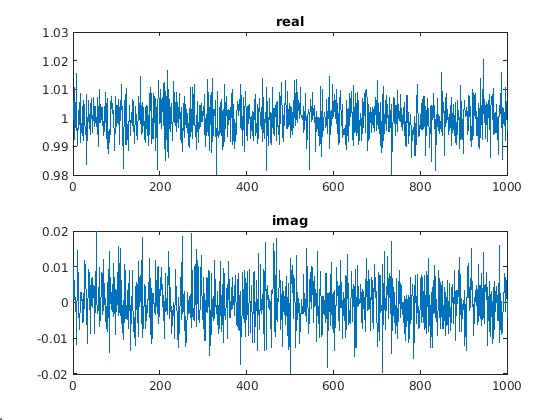
\includegraphics[scale=0.6]{b5}

The results provided are pretty close to the real value of $\theta$, but we can observe some variance in the results, which is caused by the estimation error incurred in different realizations due to the noise.

\subsection{Question 6}
Code:
\begin{verbatim}
function [] = plot6(N)
  n=(1:N)';
  K=1000;
  thetas = zeros(K, 1);
  for c=1:K
    noise=randn(N, 1) + rand(N, 1)*i;
    noise=noise./abs(noise);
    x=A*cos(2*pi*fd.*n + 1) + noise;
    thetas(c) = estimate(n, x, fd);
  end
  plot(abs(thetas))
  N
  bias=mean(thetas')-1
  variance=var(thetas')

% Execute
hold on
b6(100)
b6(1000)
b6(10000)
\end{verbatim}

Graph (blue represents $N=100$, red $N=1000$ and yellow $N=10000$):

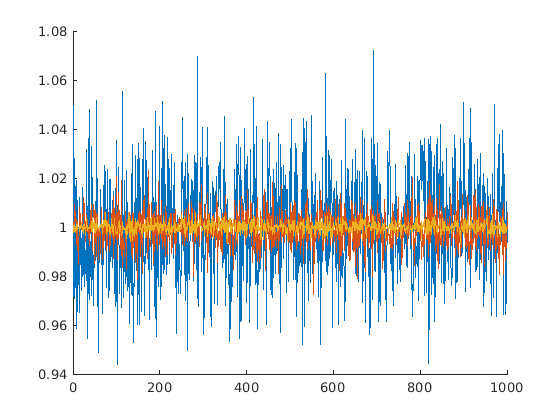
\includegraphics[scale=0.6]{b6}

Bias and variance results:
\begin{center}
  \begin{tabular}{ c c c }
   N & Bias & Variance \\ 
   100 & 7.0954e-04 - 1.5122e-04i & 5.4412e-04 \\  
   1000 & -4.7884e-04 + 1.4569e-04i & 5.8087e-05 \\  
   10000 & -9.5291e-05 - 1.3311e-05i & 5.4140e-06  
  \end{tabular}
\end{center}

It's easy to see that as $N$ grows both bias and variance decrease, meaning that, on aggregate, the higher $N$ is, the closer our estimations will be to the real value.


\subsection{Question 7}
Given that $\sigma_w = 1$ due to the fact that we imposed that on question 1, we'll get that $CRLB=\frac{2}{NA^2}$:

\begin{verbatim}
  nn=10:100:10000;    
  MSEs = zeros(length(nn), 1);
  CRLBs = zeros(length(nn), 1);
  for N=nn
    n=(1:N)';
    K=1000;
    thetas = zeros(K, 1);
    for c=1:K
      noise=randn(N, 1) + rand(N, 1)*i;
      noise=noise./abs(noise);
      x=A*cos(2*pi*fd.*n + 1) + noise;
      thetas(c) = estimate(n, x, fd);
    end
    bias=mean(thetas')-1;
    variance=var(thetas');
  
    c=ceil(N/100);
    CRLBs(c)=2/(N*A^2);
    MSEs(c)=real(bias)^2+variance;
  end
  hold on
  plot(nn, MSEs)
  plot(nn, CRLBs)
\end{verbatim}


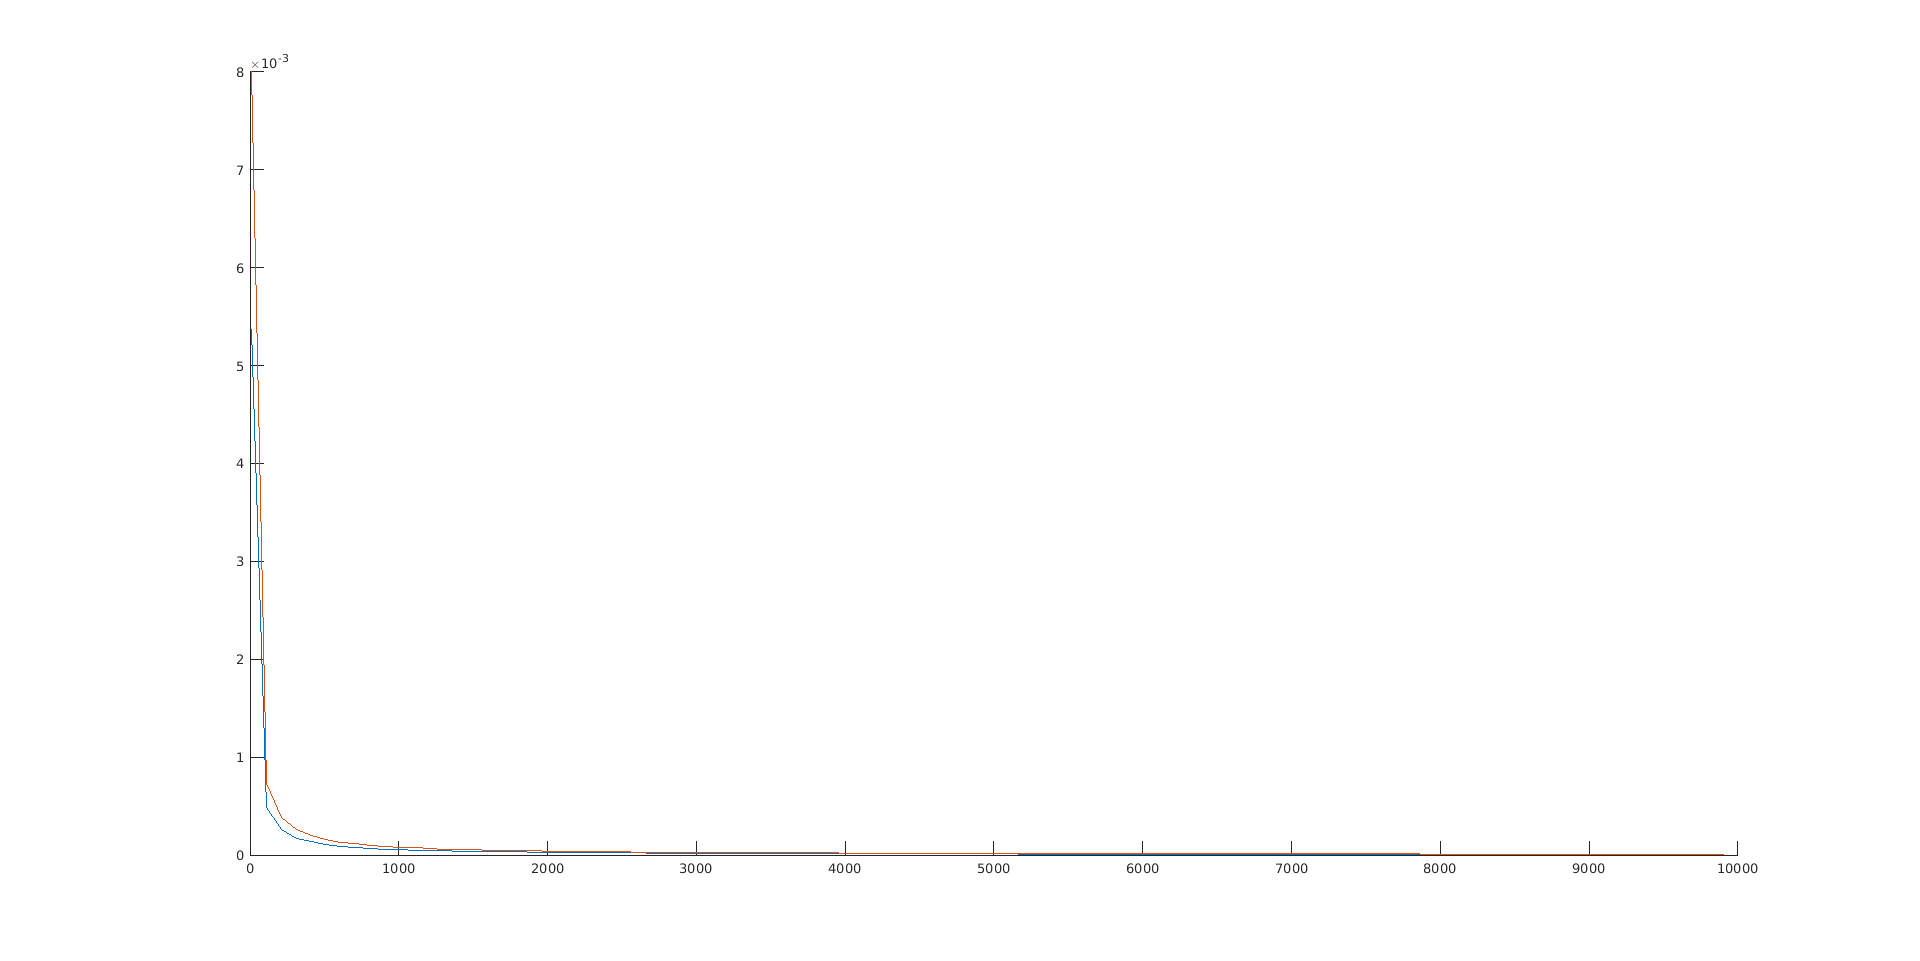
\includegraphics[scale=0.20]{b7}

On this plot we can observe that our MSE follows closely the CRLB, meaning that our predictions are quite good as they are close to the theoretical optimum, thus our ML estimator must be efficient.

Furthermore, we can appreciate how both MSE and CRLB increase sharply when getting close to really low values of N such as $10$ whereas they both decrease for larger values. This is in line with the reality, as a higher $N$ implies more data points that make it much harder for an anomaly to cause an estimation error. On the other side, if the number of data points is really low the probability of noise misleading the estimator is much higher since it's much harder for the noise to even itself out.

Finally, we can also conclude that the ML estimator is consistent, as it's bias stays generally quite low.

\end{document}


